\documentclass{IEEEtran}

\usepackage[utf8]{inputenc}
\usepackage[english]{babel}
\usepackage{graphicx}
%\usepackage[margin = 1in]{geometry}
 
\usepackage{biblatex}
\addbibresource{sources.bib}

\title{ET4394 Wireless Networking - Analyzing CRC faults}
\date{\today}
\author{
Bart Rijnders - 4103505 \\
Bernard Bekker - 4221656 
}

\begin{document}

\maketitle

\section{Abstract}

In this report the effect of signal strength, frequency and data rate on the amount of CRC failures in WiFi networks is analyzed. (insert resultaten)


\section{Hypotheses}

Packet loss can occur when the signal to noise ratio is insufficiently high to sustain communication at a certain datarate, or when two WiFi packets collide \cite{4509719}. 

\subsection{SNR vs CRC}
We expect to see a quick dropoff when the signal-to-noise ratio drops below the required SNR value.

\subsection{packet length}
Since the chance of a bit error occuring is equal for each bit in the packet. We expect the chance of a crc error to increase with $P(biterror)^{length}$. 

\subsection{errors by channel}
We expect to see a difference in errors on different channels, based on their frequency and depending on how busy they are.

\subsection{datarates}
We expect to see a higher amount of errors when seeing a low signal combined with a high datarate. For a consistent signal strength, a lower datarate should result in less errors. However, this can result in a higher chance of collisions as airtime increases \cite{4215626}. 

\section{Methodology}

WiFi packets are captured on a laptop using an intel wireless dualband-AC 8265 network adapter. Other methods attempted to capture packets include an Alfa awus036ac external wifi adapter, and a C.H.I.P. ARM devboard with build in wifi. The network adapter was placed in monitor mode using the airmon-ng application, and TShark was used to capture only data packets. A python script was written for changing the channel every 5 seconds. Approximately 1M packets are captured in lecture halls, and 1M packets in a flat building. All data is processed in Python using pandas and matplotlib.


\section{results}

\subsection{signal strength versus crc errors}

Some interesting aspects can be seen in figure \ref{fig:totalpackets}. The good reception at high signal strengths, a strong dropoff after a certain point, and two main dips in the reception of correct packets. The most starteling aspect is the rise in correctly received packets at even lower signal strength. We can see more patterns if we split the results into 2.4Ghz channels, and 5.8 Ghz channels (fig \ref{fig:24packets} and fig \ref{fig:58packets}). The two dips are explained by the different dropoff points for 2.4 Ghz and 5.8Ghz. Because 5.8Ghz has less noise, the packets can be correctly demodulated at a lower signal strength.

\begin{figure*}[tb]
		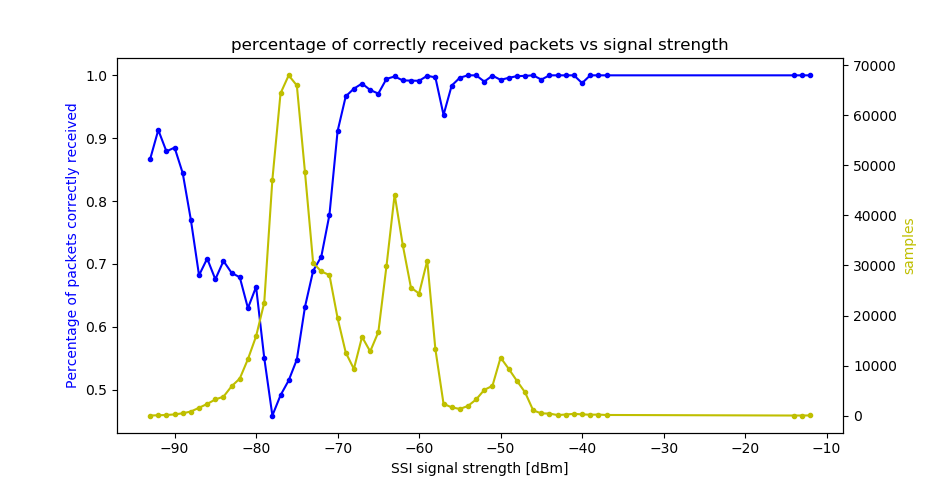
\includegraphics[width=\textwidth]{figures/packets_total.png}
		\caption{A total overview of crc error rates in packets versus signal strength. The blue line shows the portion of messages being received without a crc error. The yellow line show the amount of samples at each data point. }
		\label{fig:totalpackets}
\end{figure*}

\begin{figure}
		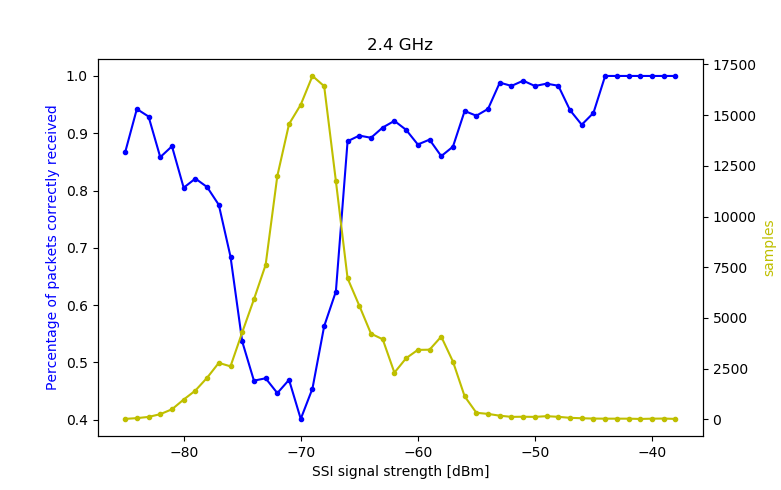
\includegraphics[width=0.5\textwidth]{figures/24ghz.png}
		\caption{}
		\label{fig:24packets}
\end{figure}

\begin{figure}
		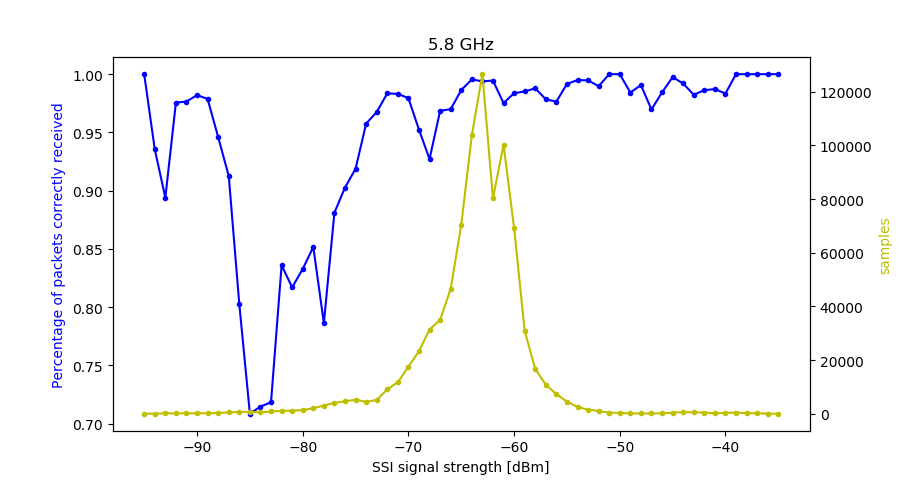
\includegraphics[width=0.5\textwidth]{figures/58ghz.png}
		\caption{}
		\label{fig:58packets}
\end{figure}

This leaves to explain why the graph turns up again at very low signal strenghts. We expect this to be a result of this experiment not being a controlled experiment. Since we do not have a control of what packets are being send, the results only show the packets that are received by the network adapter. When the signal deteriorates too far, it is no longer forwared to the driver and OS. We can see this clearly in fig \ref{fig:datasignal}. At low signal rates, only the packets with a low datarate are returned (As expected due to Shannon's law). This implies that we should see a tradionional curve when we isolate a single datarate, and this is confirmed when isolating a single datarate in fig \ref{fig:singledatarate}.

\begin{figure*}
		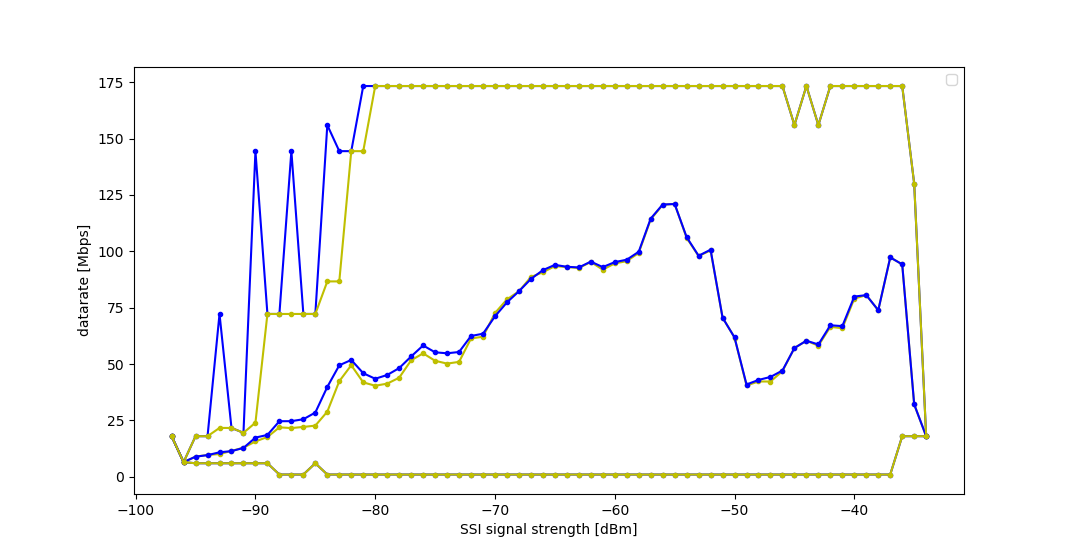
\includegraphics[width=\textwidth]{figures/datarate_signal.png}
		\caption{maximum, mean and minimal reported datarates of received packets vs. signal strength. The blue line is the datarate of all received packets, the green line the datarate of packets without CRC errors. At low signal strenghts, all lines converge as the network adapter drops all undecipherable packets and only shows packets that are succesfully received due to their low datarate.}
		\label{fig:datasignal}
\end{figure*}

\begin{figure}
		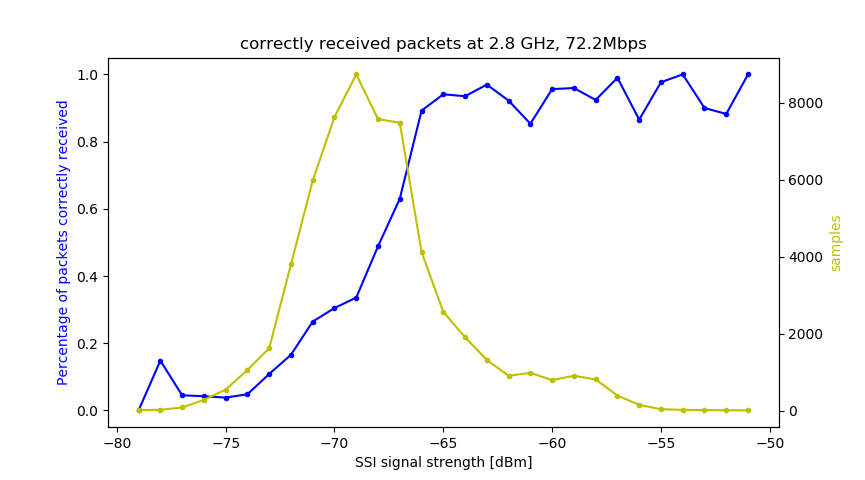
\includegraphics[width=0.5\textwidth]{figures/24ghz72mbps.png}
		\caption{}
		\label{fig:singledatarate}
\end{figure}

\subsection{Packet length}

Contrary to our expectations, the relation between packet length and the error percentage seems not to be exponential. While hard to exactly pin down a correlation, it seems to be mostly linear. This can be explained by the devices communicating adapting the settings of the channel to keep the error rate low. In the prior work \cite{7317401}, the authors saw a constant error rate with increasing packet length, but an increase in error rate when increasing the airtime. However, this seemed mostly constant in our datasets (see fig \ref{fig:airtime}). 

\begin{figure}
		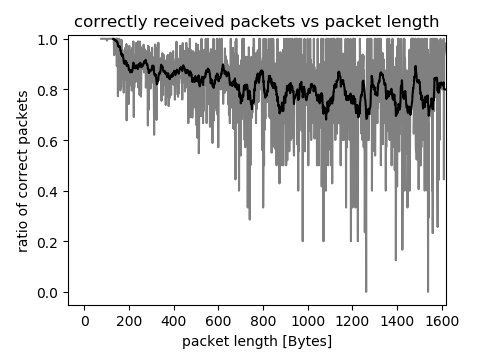
\includegraphics[width=0.5\textwidth]{figures/length.png}
		\caption{Percentage of packets without error versus packet length.}
		\label{fig:length}
\end{figure}

\begin{figure}
		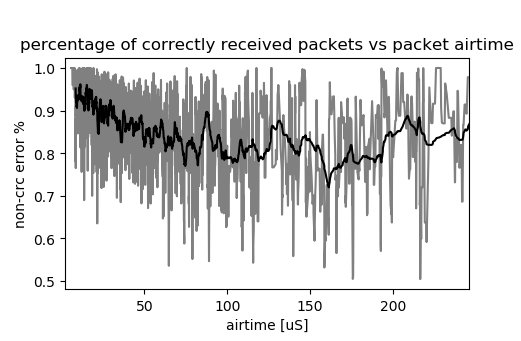
\includegraphics[width=0.5\textwidth]{figures/airtime.png}
		\caption{Percentage of packets without error versus airtime.}
		\label{fig:airtime}
\end{figure}


\subsection{channels}
\begin{table}[f]
\centering
\caption{packet success rate in a flat building}
\label{my-label}
\begin{tabular}{lll}
Channel & \% successful packets & Samples \\
1       & 0.98                          & 352763  \\
5       & 0.52                          & 277195  \\
6       & 0.67                          & 99189   \\
9       & 1.0                           & 3237    \\
44      & 1.0                           & 415    
\end{tabular}
\end{table}

\begin{table}[f]\centering
\caption{packet success rate in a university lecture hall}
\label{my-label}
\begin{tabular}{lll}
Channel & \% successful packets & Samples \\
1       & 0.96                          & 352763  \\
5       & 0.52                          & 277195  \\
9       & 0.84                          & 99189   \\
44      & 0.99                          & 3237   \\
48      & 0.80                          & 415    \\
60      & 0.95                          & 1425   \\
100     & 0.96                          & 137178 \\
\end{tabular}
\end{table}
\subsection{datarate}
Our data shows few crc errors for both high and low datarates at high signal strengths (fig \ref{fig:datasignal}). At critical signal strengths, the average datarate of packets without an error is slightly lower than for all packets. At low signal strength, only packets with a low datarate are received by the network adapter. This is consistent with our expectations.

\section{discussion}

Our ability to get good results was hindered by the capabilities of our hardware. We were not able to perform an experiment in an controlled situation, and could not quantify the noise floor during our measurements. For some reason, our capturing laptop completely ignored the packets send by some devices, but did show the packets of others. Even when connected to the same access point.


\clearpage
\printbibliography

\end{document}